% !TEX root = ../../prj4projektrapport.tex
% SKAL STÅ I TOPPEN AF ALLE FILER FOR AT MASTER-filen KOMPILERES 

\subsection{Software}
I dette afsnit vil design og implementering af softwaren på PSOC blive beskrevet. Herunder sampling af signaler, Fourier beregninger og  UART kommunikation. For detaljeret beskrivelse af softwaren henvises til dokumentationen\footnote{Projektdokumentationen, 9.2, Software}

\subsubsection{Overordnet beskrivelse}
Det overordnede flow i koden er beskrevet i Figur \ref{fig:MEflowchart}. 

Ved start af Måleenheden sker der en række initieringer af interrupts og blokkald. Herefter ender koden i en uendelig loop, uden aktivitet. Ved modtagelse af data over UART forbindelsen aktiveres en interruptrutine, hvor hovedparten af kodens funktionalitet er allokeret. 
Afhængigt af hvilken karakter der er modtaget på UART forbindelsen udførers forskellige instruktioner. I følge protokollen for UART-forbindelsen modtages karakterene A-B-C-D, i rækkefølge. (REFERENCE)
Når den første karakter A er modtaget påbegynder måleneheden sampling af signalerne, hvorefter værdien for strøm sendes tilbage over UART forbindelsen. Herefter afventes de resterende receive interrupt, som giver anledning til at spænding, THD, og power faktor sendes til Styringsenheden. 
\begin{figure}[H] % (alternativt [H])
	\centering
	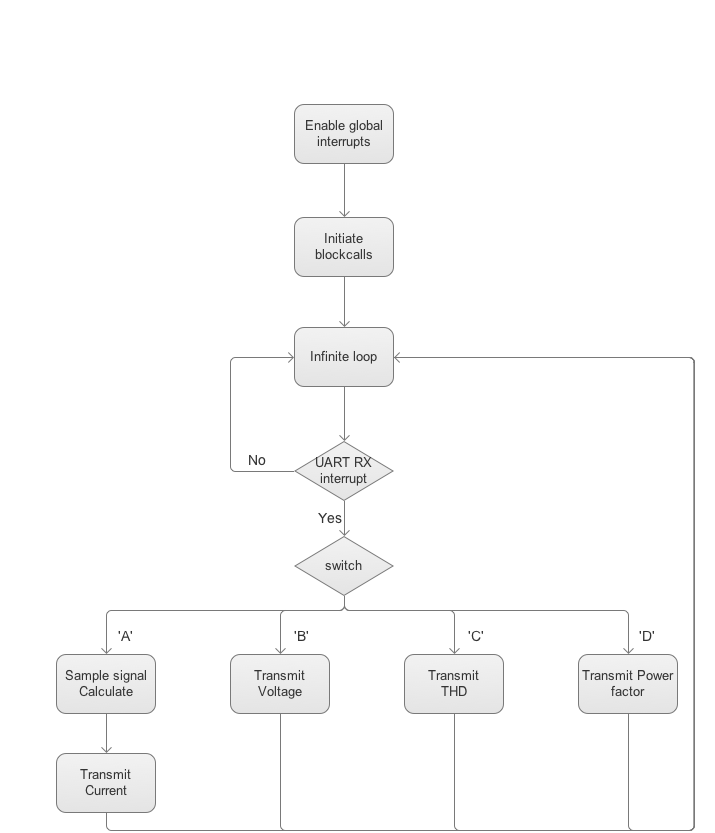
\includegraphics[width=0.7\textwidth]{Figure/MEflowchart.png}
	\caption{Overordnet flowchart for software på Måleenhed}
	\label{fig:MEflowchart}
\end{figure}
